\section{From Tacit to Explicit:\newline{}Theoretical and Conceptual Framework}

\subsection{Of Science \& Technology Studies}

While activities in hackerspaces are assorted and quite diverse, the common denominator in terms of interests and pursuits seems to be overwhelmingly related to technology, mostly having to do with computer hardware and software, electronics and mechanics. A recent survey of hackerspaces published by Finnish researcher Jarkko Moilanen \citeyearpar{moilanen10} (who, incidentally, is doing his PhD Thesis in the topic of hackers and activism ---\textit{hacktivism}) revealed that computer software and hardware development were by far the most popular activities performed in hackerspaces. Thus, examining the hackerspace phenomenon from the perspective of the field of Science and Technology Studies (S\&TS) intuitively seemed like a good choice in need of further exploration.

Science and Technology Studies refers to the impact that social values and circumstances have on scientific research and technological development. As an interdisciplinary subfield of sociology, it has its origins in the wider series of revolutions that took place during the 1960s. \citet{edge95} describes its genesis in a ``number of well-established specialities in history and philosophy \ldots sociology, anthropology and \ldots in economics and the political and legal sciences'' \citep[p.4]{edge95}. It ``came of age'' as a unified discipline, however, as a result of the work of Thomas Kuhn \citeyearpar{kuhn62}. Kuhn's research on the social (and somewhat volatile) nature of scientific knowledge-building and his concept of \textit{scientific paradigms} served both as a founding platform and as a source of inspiration for what would become S\&TS. 

Also important in establishing the discipline was a widespread institutional quest for ``a rational basis for science policy'' \citep{edge95} in the United States during the 1960s, motivated by the revelation of Nazi atrocities in the name of science as well as the developments of the cold war, both of which converged to reinforce the stereotype of the ``mad scientist'' \citep{frayling05}\footnote{These events were masterfully immortalised by Stanley Kubrick's 1962 classic \textit{Dr. Strangelove or: How I Learned to Stop Worrying and Love the Bomb}.} as well as the rise of a collective ``heightened awareness'' by the baby-boom generation around that same time. These factors played important roles in uniting a series of scholars who, up until that moment, had worked in relative isolation in coming up with the S\&TS (formerly STS) label \citep{kaplan91}.

Since then, S\&TS has become a universally recognised field as evidenced by the growing number of university programmes and departments as well as scholarly publications \citep{besselaar00}. As it relates to this project, S\&TS is particularly valuable as it seeks to understand how society shapes the development of science and technology, rather than the effects of science and technology on society. As I argue next, this outside-to-inside approach is particularly insightful in studying hackers and hackerspaces.


\subsection{A Triad of Relations}

This project focuses on three major relationships that take place inside hackerspaces, which I have decided to name \textit{socialising}, \textit{learning} and \textit{making}. I view these relationships as ordered (yet simultaneous) steps in the creative processes that ---I hypothesise--- can lead to meaningful innovation. As detailed in section \ref{structure}, these three relationships will comprise the core of this dissertation.

In attempting to answer my research questions and having located my project within the discipline of Science and Technology Studies, I will build on the work of Michael Polanyi \citeyearpar{polanyi58,polanyi66}, particularly on his concept of \textit{Tacit Knowledge}, which states that knowledge (its acquisition and transmission) is composed of both tacit and explicit components, the latter not being able to exist without the former\footnote{See more about Polanyi and tacit knowledge in section \ref{polanyi}}.

Like Thomas Kuhn, Polanyi also insisted that knowledge is indissolubly tied to social networks and circumstances, opposing the then-prevail\-ing positivistic view of scientific knowledge, whereby it was supposed to advance linearly, as a result of increasingly accurate measurements of empirical data. I adopt Polanyi as a governing theorist ---and not Kuhn--- for a number of reasons, first of which is the fact that Polanyi's work is meant to be taken as an all-encompassing epistemological system, applying not only to formal scientific research but to a much broader scope of phenomena. While Kuhn's model can be applied to areas outside science, \textit{The Structure of Scientific Revolutions} deals specifically with formal, established scientific methodologies. Indeed, as noted by \citet{gutting84}, Kuhn explicitly noted that his ideas were only intended to apply to natural sciences. Furthermore, as \citet{laudan84b} notes, it is ``transparently clear that technology transfer is very hard to achieve'' due to its tacit nature. Thus, I believe, Polanyi's model is better suited to examine the broader notions of \textit{learning} and \textit{making}, particularly outside formal academic or scientific environments.

Secondly, while one of my hypotheses is that hackerspaces are suitable (in fact, ideal) places for research and development, it would be unrealistic for me to expect to witness any ``revolutionary'', ``paradigm-shifting'' activities during the course of my research, rather observing what Kuhn calls the practice of ``normal'' science\footnote{I use the term ``science'' quite broadly in this context. A more accurate term would be ``normal technological research'' as understood within the field of S\&TS. See \citet[p.75--85]{sismondo04}} \citep[p.10]{kuhn62}, for which Polanyi is better suited.

All three of my core chapters ---each examining and developing the notion of a different relationship: \textit{socialising}, \textit{learning} and  \textit{making}--- will be grounded atop three complementary sub-frameworks, with which I will attempt to solve the specific questions each one raises while maintaining coherency with the dissertation's overall theme.

\subsubsection{Interaction Ritual Theory}

Chapter four, \textit{socialising}, will build on \citepos{durkheim12}, \citepos{goffman67} and \citepos{collins04} work with regards to rituals, particularly Collins' \textit{Interaction Ritual Theory}. Using IRT, I intend to analyse the social structure of hackerspaces in terms of power relationships and group dynamics by looking into hackers' everyday micro rituals. I use the term ``ritual'' in the way proposed by Collins, who distances it both from its popular and anthropological meanings, instead using \citeauthor{goffman67}'s definition as a starting point, whereby it is ``found in one degree or another throughout everyday life; in the secular realm as in the sacred and official worlds, [it] plays a key role in shaping both individual character and stratified group boundaries'' \citep[p.8]{collins04}.

According to the author, IRT attempts to make sense or ordinary ``micro-rituals'', or microsociological events, by placing emphasis in ``the process in which participants develop a mutual focus of attention and become entrained in each other's bodily micro-rhythms and emotions'' \citep[p.47]{collins04}. His theory identifies a set of causes and effects (ingredients and outcomes) that converge to make sense of successful rituals. 

Ingredients for successful rituals include
\begin{inparaenum}[\itshape a\upshape)]
  \item \textit{bodily co-presence}, whereby participants physically converge in a single space and ``affect each other by their bodily presence'' \citep[p.48]{collins04},
  \item \textit{barriers to outsiders} that define clear boundaries for the group, and
  \item what the author calls \textit{mutual focus of attention} and \textit{shared mood} by which participants devote their attention to single, specific events which in turn provide them with some sort of satisfactory outcome.
\end{inparaenum}

In turn, these ingredients cause successful rituals to reach a number of outcomes:
\begin{inparaenum}[\itshape a\upshape)]
  \item group solidarity,
  \item emotional energy,
  \item sacred objects or symbols that represent the group\footnote{Just as \citeauthor{goffman67} before him, \citeauthor{collins04} suggests that these can be inanimate artefacts, other human beings and other creatures, amongst other things.}, defended and treated with great respect and
  \item common standards of morality, which delineate the boundaries of accepted behaviour within the group.
\end{inparaenum}


Using interaction ritual theory, I intend to understand how social relationships are fostered inside hackerspaces and how those relations ultimately kick-start the learning and knowledge-transmission processes. I hypothesise IRT's necessary corporeality and its capacity to affect ritual participants (hackers) manifests itself as and ultimately leads to the successful initiation of the transmission of tacit and explicit knowledge.

I will also attempt to make sense of the hackerspace phenomenon by examining how it relates to interaction ritual theory's other conditions and outcomes, while pointing any potential divergences from Collins' original theory. Of crucial importance are concepts of trust and acceptance.

\subsubsection{Legitimate Peripheral Participation in Communities of Practice}

For chapter five, \textit{learning}, I intend to build on the conclusions of the previous chapter, namely how hackers' power relationships and group dynamics foster a learning environment and apply Jean Lave and Etienne Wenger's \citeyearpar{lave91} notions of \textit{Legitimate Peripheral Participation} within \textit{Communities of Practice} in order to attempt to understand how the learning and knowledge transmission process takes place, all while viewing it from the perspective of Polanyi's tacit knowledge.

\citeauthor{lave91} expand and enhance the concept of apprenticeship to describe how groups and communities learn from each other by means of practice and social interaction. Like Kuhn and Polanyi, the authors view the learning experience as a social journey ---in their case from ``newcomer'' to ``old-timer'' \citep[p.56--57]{lave91} within a social construct they have named communities of practice. The authors argue that members ``socially negotiate'' their positions (by means of conflict, interaction and participation) while becoming more relevant and essential to their group. By doing so, they learn their trade and skills by means of direct interaction with other members of their group. Legitimate Peripheral Participation is, thus, aimed at understanding how social circumstances influence shape and facilitate the learning process. It is \emph{not} a pedagogical strategy or a learning technique.

The authors attempt to make sense of the nature of learning within relatively small, specialised groups (tailors, midwives and, as would be my case, hackers) by analysing the paths by which novices become experts, mastering the tricks of their specific trades by imitating and maintaining contact with senior members in circumstances where real-world nuances such as conflict, envy and scarcity of resources have palpable effects. These pathways describe movement from a \textit{peripheral} state to an ideal one of \textit{full} participation. Further, on-going pathways from peripheral to full participation lead to what the authors dub \textit{reproduction cycles} inside these communities: new members gain expertise while older ones ultimately retire, sustaining the same processes for long periods of time. While physical co-presence is not explicitly required in LPP, the authors certainly suggest that mutual spatiality exhibits numerous benefits.

Applying LPP to my work, chapter five will start by looking at individual hackerspaces (at three different locations) and examine them as single, independent communities of practice, considering the fact that, while, rhetorically, anyone is welcome at most hackerspaces, newcomers will face barriers of entry (to be identified in the earlier chapter) which they will have to overcome (partly, I speculate, by acquiring new skills) to increase the value of their roles within each hackerspace. Lave and Wegner note that, while the term ``peripheral'' is not to be taken as something negative, the process of increasing one's position (gaining acceptance) is not an easy task. Power relations as examined in the previous chapter will serve as a starting point in examining the master-apprentice communion, one of Lave \& Wenger's essential relations in the learning process.

\subsubsection{Cognitive Change Theory}

Chapter six, \textit{making} will seek to understand how the processes described in the previous two chapters ultimately lead to valuable innovation. I will do so by using \citepos{laudan84} problem-solving model of technology. Laudan places problem-solving at the centre of the technological innovation process. In her analysis, problem-solving constitutes an all-encompassing activity, dealing not only with utilitarian and perhaps mundane aspects, but also including ``the fun \ldots the aesthetic and intellectual issues that engage the practitioner'' \citep[p.84]{laudan84}, which, as demonstrated by \citepos{moilanen10} survey, seems to fit hackerspaces quite well.

\citeauthor{laudan84} proposes five categories of ``problems'' which, when addressed technically, stimulate the advance of technology. The first one, ``problems not yet solved by any technology'' is also said to be the least common. Second is what the author calls ``functional failure of current technologies'', while the third is stated as ``extrapolation from past technological successes''. Fourth are ``imbalances between related technologies'' whereby strong innovation on one end requires and stimulates the other to ``keep up'', while the fifth category has to do with foreseen or potential failures in current technologies, for instance, a future scarcity of hydrocarbon-based fuel sources.

Laudan's model also describes three levels of technological knowledge, which, in order of complexity, are categorised as individual technologies, complexes and systems. Summarily, individual technologies are isolated solutions that address single and distinct problems. Complexes are coherent combinations of individual technologies in symbiotic relationships\footnote{Aircraft, with their propulsion, guidance and other mechanisms are good examples of complexes}, while systems are ``epochs gradually replacing one another'' \citep[p.92]{laudan84}\footnote{The bronze age or the industrial revolution would be examples of systems}. 

By making problem-solving the cornerstone of technological innovation, the author raises a number of interesting questions. Abundance of problems, for instance, will require practitioners to develop a criteria for selecting which problems to address. Furthermore, she suggests that, as inter-related problems are selected, a process of ``niche-isation'' occurs within communities of technological practice. Such niches present a formi\-dable opportunity for a comparison-based analysis of multiple hackerspa\-ces and the environmental effects of their localities.

%\begin{center}
\begin{figure}[ht]
	\centering
		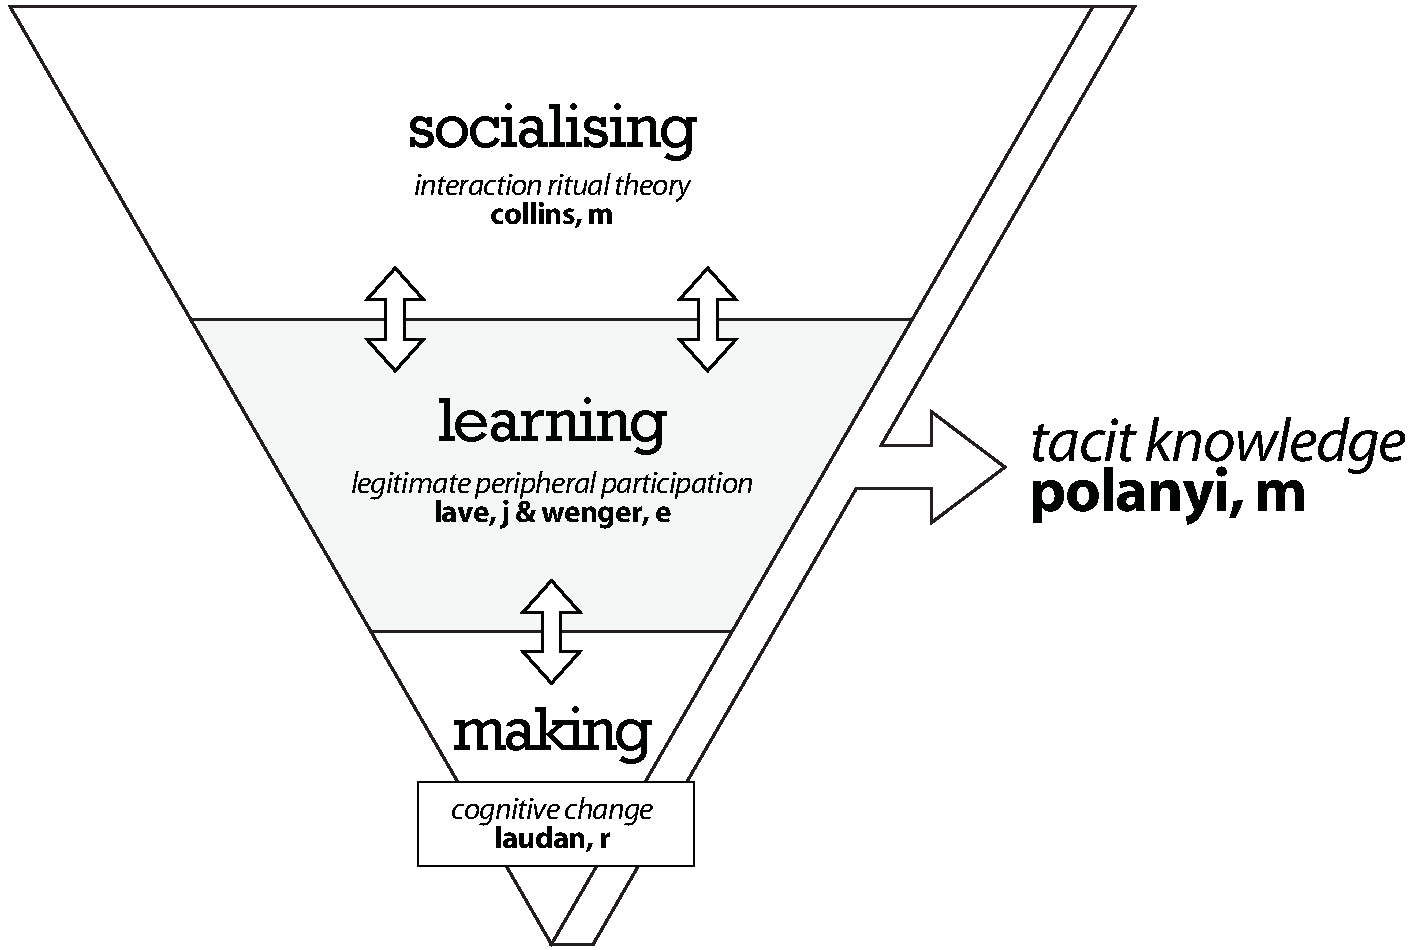
\includegraphics[scale=0.45,natwidth=10pt,natheight=1pt]{confirmation-report/graphs/pyramid01.pdf}
	\caption[Theoretical Relations]{Graphic relationship between theoretical approaches}
	\label{pyramid}
\end{figure}
%\end{center}

It is important to note that I do not see my three core chapters as independent, self-sustaining units. Rather, I regard their relation as a type of funnel-like structure or an inverted pyramid, going from broad to specific, from the everyday generalities of human contact to the much more unusual breakthroughs of value-adding innovation. Figure \ref{pyramid} aptly illustrates the reasoning behind the theoretical relations that will sustain the core of my dissertation, which have also heavily shaped my proposed methodological approach, described in more detail in section \ref{methodology}.

\newpage


 

\section{Thesis Structure}
\label{structure}

The macro-structure of my dissertation will be organised according to what \citet{dunleavy03} calls a ``compromise model'', emphasising the core research chapters (informally referred to as ``the beef'' by the author), without disregarding the always necessary lead-in chapters. Figure \ref{structure-graph} presents a schematic model of my proposed structure, detailing relative lengths of each chapter and macro sections with relation to the whole and providing a summarised view of each chapter.

%\begin{center}
\begin{figure}[ht]
	\centering
		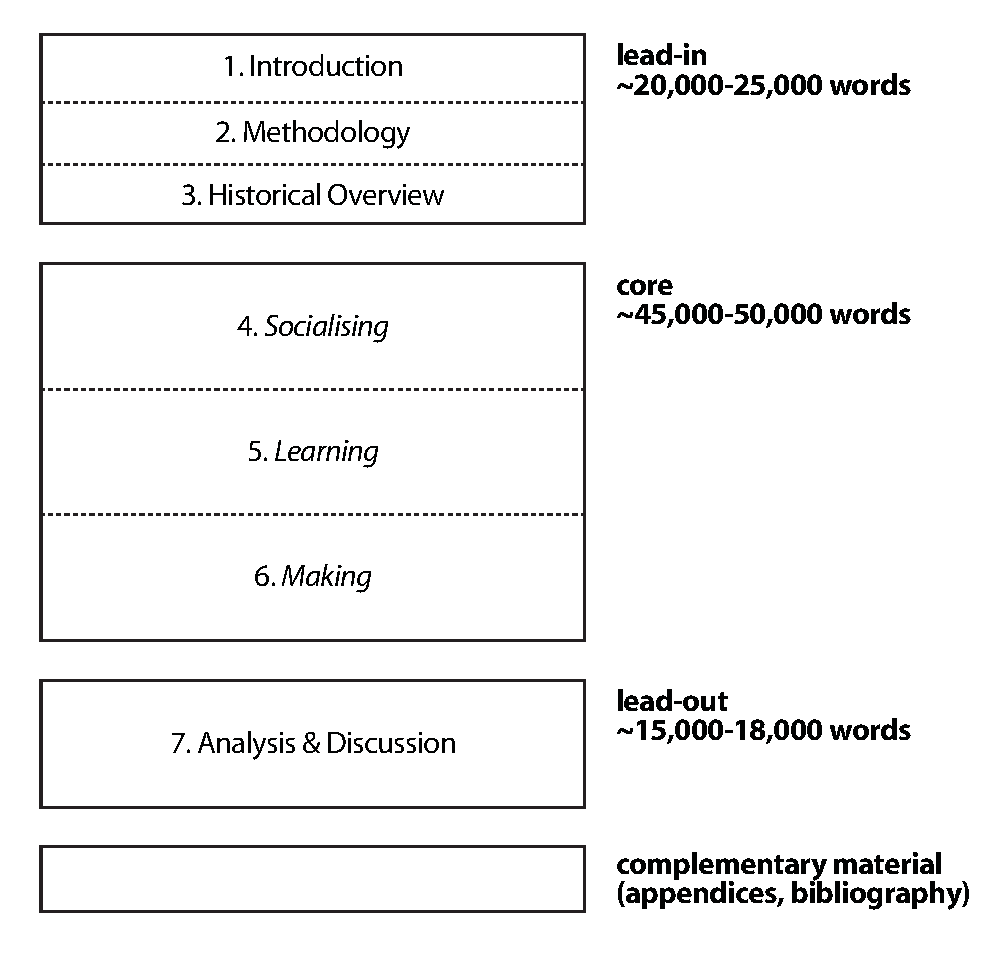
\includegraphics[scale=0.65,natwidth=10pt,natheight=1pt]{confirmation-report/graphs/structure01.pdf}
	\caption[Thesis Structure]{Theoretical structure of the dissertation's three core chapters}
	\label{structure-graph}
\end{figure}
%\end{center}


As mentioned above, the core of the dissertation will be divided into three chapters, each revolving around a different but complementary relationship and theoretical framework. Chapter 4, \textit{socialising}, will look at hackers' everyday rituals taking place inside hackerspaces using \citepos{collins04} interaction ritual theory. Chapter 5, \textit{learning}, will attempt to understand how social relations amongst hackers influence and facilitate their learning and transmission of technical skills. It will do so building upon \citepos{lave91} concepts of Legitimate Peripheral Participation and Communities of Practice. Further, Chapter 6, \textit{making} will seek to examine whether such skills can ultimately yield innovation in the form of valuable technological contributions. It will do so based upon \citepos{laudan84} model of Cognitive Change.

Present throughout the entire dissertation will be \citepos{polanyi66} concept of Tacit Knowing, attempting to make sense of the wider epistemological concern regarding the importance of physical presence in knowledge transmission. All three chapters will be supported by ethnographic data collected by means of participant observation and intensive interviewing in Melbourne, San Francisco and Bogot\'{a}.

Complementing the core macro section, chapter 2 will present a detailed account of the research design, the obtained data and a comprehensive rationale for each of the decisions made as a result of the research process. It will also attempt to report my experiences in the field: shortcomings, successes, rewards and any other eventualities. Chapter 3 will delve into the history of hackers and hackerspaces, providing much-needed context into the emergence of these communities and their members, whom I perceive as fitting into the wider category of Bohemia, all while reviewing existing scholarly literature.

Chapter 7 will provide a final analysis, discussing all findings from the perspective of tacit knowledge, examining the implications of such findings and, finally, linking them back to the existing literature, locating the contributions made by the work within its field of study.
